\section{Ontologias}
\label{sec:ontology}

Uma ontologia é uma representação formal de conhecimento sobre um domínio e está baseada na lógica de descrição. Inclui as seguintes componentes:

\begin{itemize}
	\item Tipos de entidades (e.g. Pessoa, Companhia, etc)
	\item Propiedades de entidades (e.g. nome, sobrenome, etc)
	\item Relações entre entidades (e.g. paiDe, irmãoDe, etc)
	\item Eventos que acontecem com entidades (e.g. escolher a melhor opção, etc)
\end{itemize}

Além disso, por ser baseada em lógica, existe a possibilidade de fazer inferências sobre os fatos estabelecidos nela. Também pode ser usada para ajudar os motores de busca responder a perguntas mais complexas.

\begin{lstlisting}[ caption = Uso de OWL , label = ex:owl ]
	<owl:Class rdf:ID="WineDescriptor" />
	
	<owl:Class rdf:ID="WineColor">
		<rdfs:subClassOf rdf:resource="#WineDescriptor" />
		...
	</owl:Class>

	<owl:ObjectProperty rdf:ID="hasWineDescriptor">
		<rdfs:domain rdf:resource="#Wine" />
		<rdfs:range  rdf:resource="#WineDescriptor" />
	</owl:ObjectProperty>

	<owl:ObjectProperty rdf:ID="hasColor">
		<rdfs:subPropertyOf rdf:resource="#hasWineDescriptor" />
		<rdfs:range rdf:resource="#WineColor" />
		  ...
	</owl:ObjectProperty>
\end{lstlisting}

A linguagem padrão para representar ontologias é chamado OWL (Web Ontology Language) e foi estabelecido por o World Wide Web Consortium (W3C) no ano 2004. Seu uso é mostrado no Exemplo~\ref{ex:owl} onde estão instanciadas classes, subclasses e propriedades. O problema é que manter aquela estrutura manualmente é complicado e por isso foram aparecendo ferramentas gráficas que a geram automaticamente. A ferramenta mais usada atualmente para construir ontologias é Protegé (Figura~\ref{fig:protege}).

\begin{figure}[h]
	\centering
	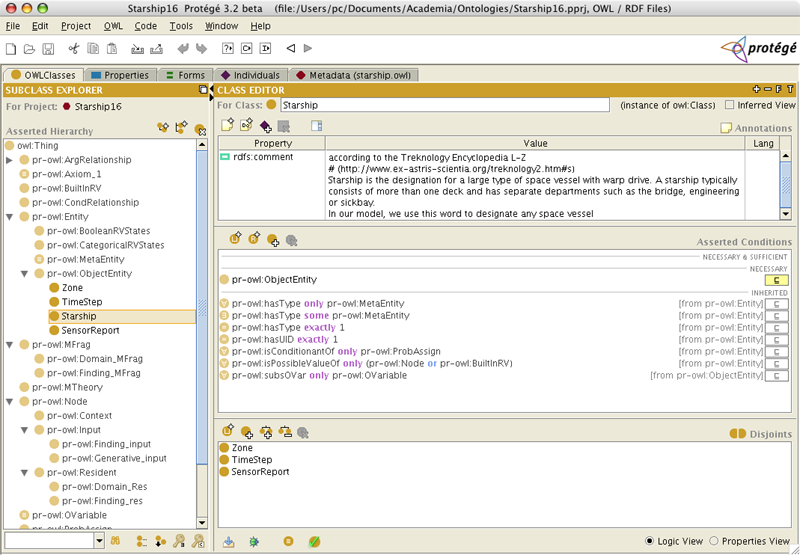
\includegraphics[height=9cm]{./images/protege}
	\caption{Protegé}
	\label{fig:protege}
\end{figure}

Mas o principal problema de usar as ontologias comuns e OWL como meios para obter a web semântica é que a web atual tem incerteza em muitos conceitos. Esta poderia estar não só em tipos de entidades (e.g. Python é uma linguagem de programação ou um animal), se não também em propriedades ou relações que tem diferentes comportamentos em diferentes domínios (e.g. limpo pode significar que não tem registros policiais, ou que não está sujo). Tendo isto em consideração, existe uma necessidade de encontrar uma representação nova que use tanto lógica como teoria de probabilidades para representar o conhecimento e também de extender a linguagem OWL para ter suporte de probabilidades.